\clearpage
\subsection{Organigrama de la Empresa}

\begin{center}
    \vspace{0.3cm}
    % Título formato APA 7
    \refstepcounter{figure}
    \label{fig:organigrama}
    \addcontentsline{lof}{figure}{%
        Figura~\thefigure.
        Estructura orgánica funcional de J\&P Periféricos S.A.C.}

    {\bfseries Figura~\thefigure}\par\vspace{0.1cm}
    {\itshape Estructura orgánica funcional de J\&P Periféricos S.A.C.}\par
    \vspace{0.20cm}

    % Organigrama con borde (ancho 0.98 para evitar advertencia de desborde de margen)
    {\color{gray!60}\setlength{\fboxsep}{0pt}\setlength{\fboxrule}{0.6pt}%
    \fbox{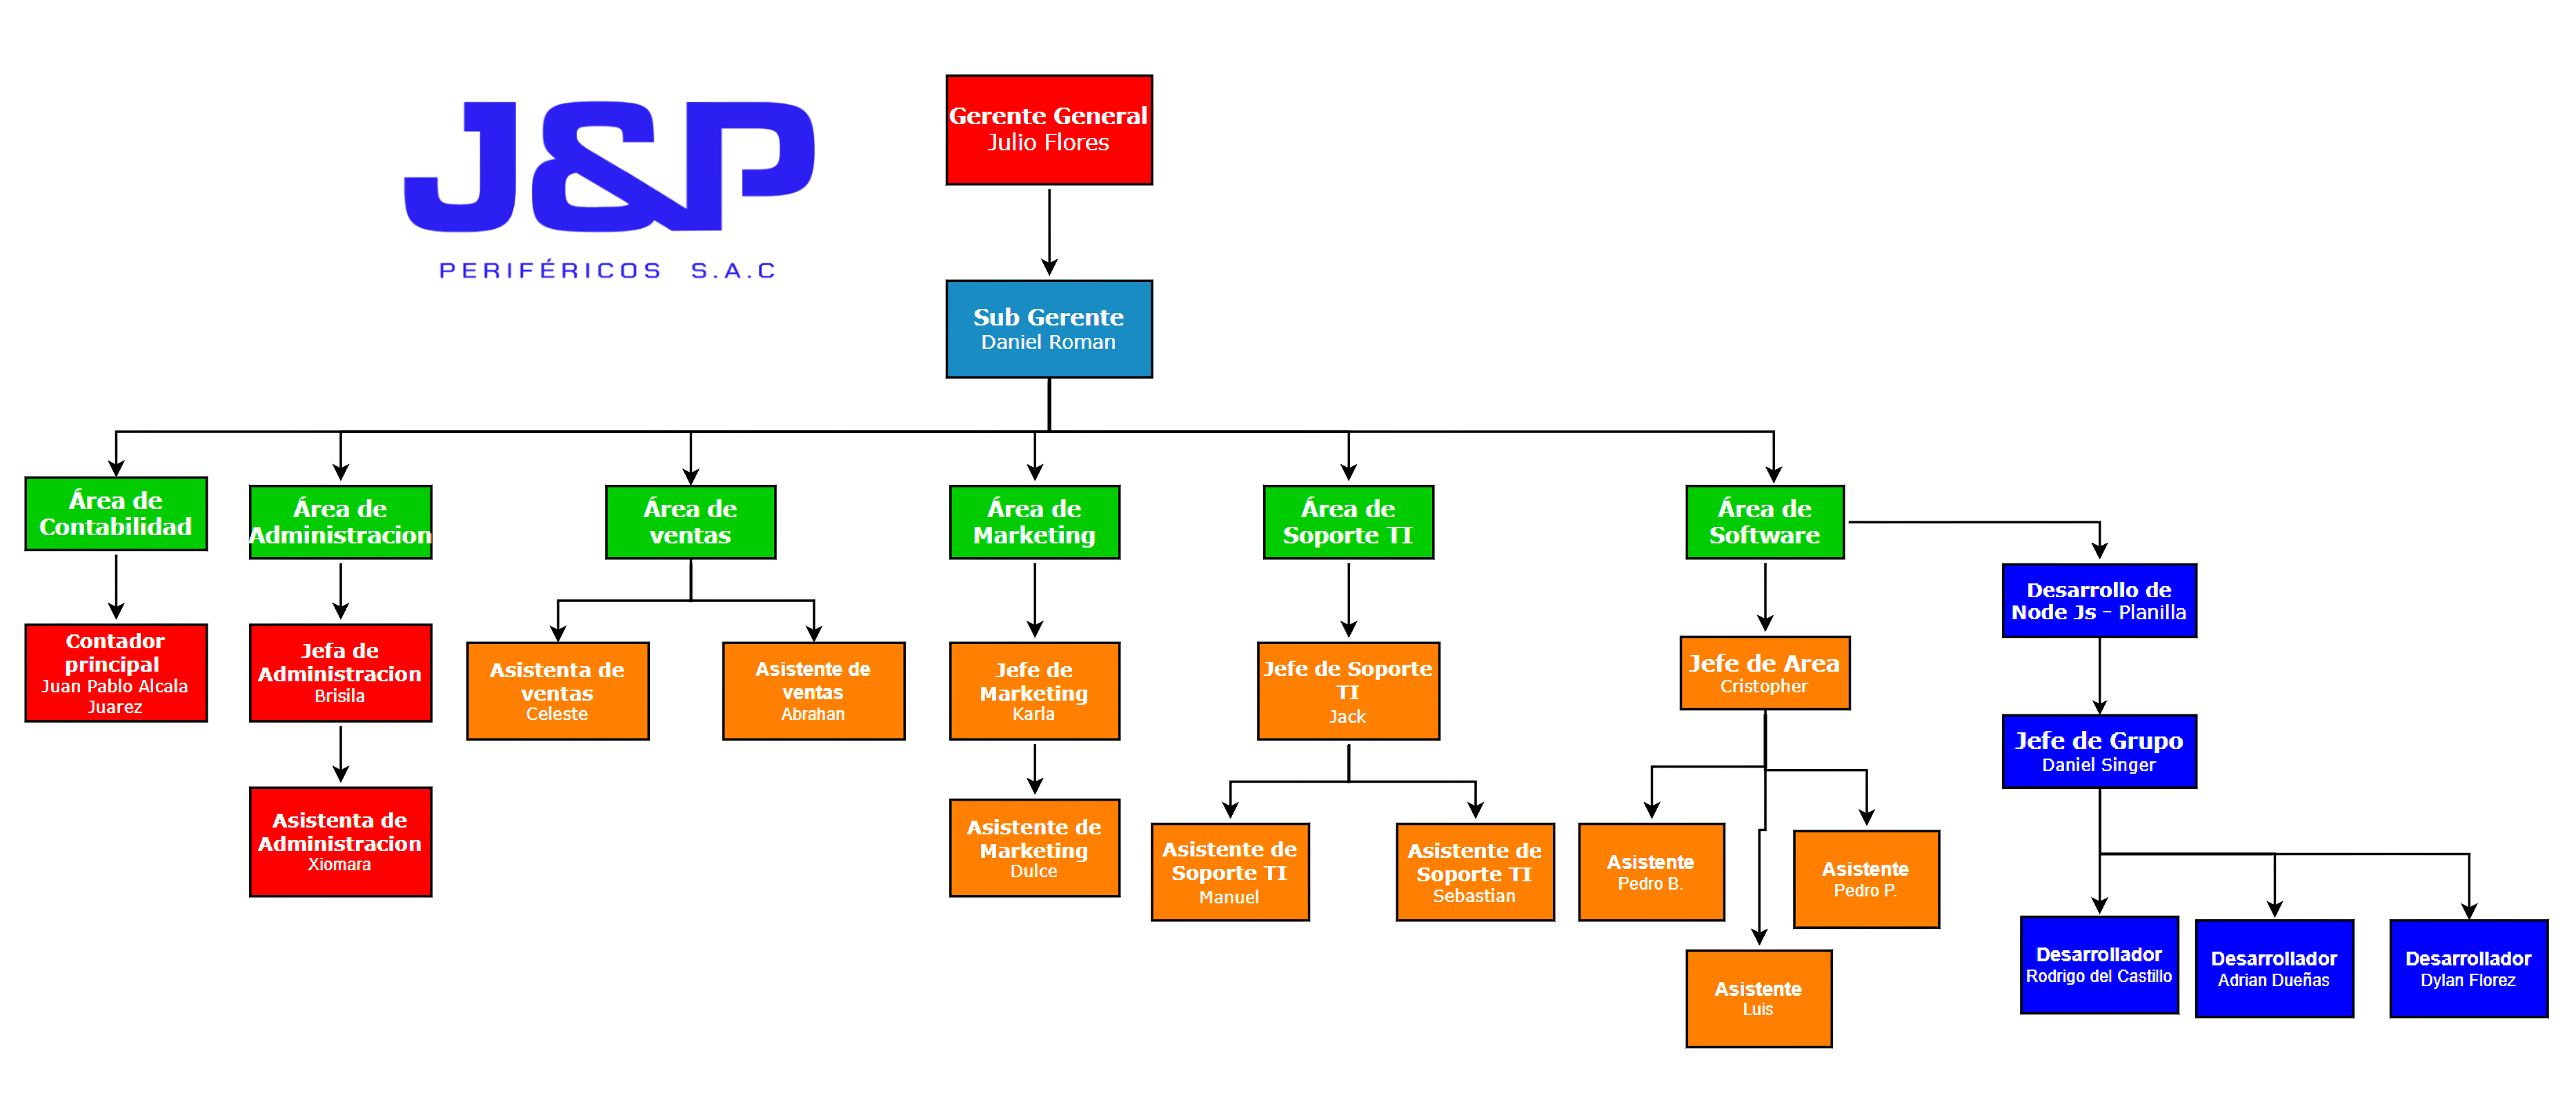
\includegraphics[width=1\linewidth]{images/organigrama.png}}}\par
    \vspace{0.25cm}

    % Nota APA 7 alineada al ancho de 0.98
    \begin{minipage}{0.98\linewidth}
        \small
        \textit{Nota.} Representación jerárquica y departamental de las áreas funcionales de la empresa. Elaboración propia.
    \end{minipage}
\end{center}
